%%%%%%%%%%%%%%%%%%%%%%%%%%%%%%%%%%%%%%%%%%%%%%%%%%%%%%%%%%%%%%%%%%%%%%
% How to use writeLaTeX: 
%
% You edit the source code here on the left, and the preview on the
% right shows you the result within a few seconds.
%
% Bookmark this page and share the URL with your co-authors. They can
% edit at the same time!
%
% You can upload figures, bibliographies, custom classes and
% styles using the files menu.
%
%%%%%%%%%%%%%%%%%%%%%%%%%%%%%%%%%%%%%%%%%%%%%%%%%%%%%%%%%%%%%%%%%%%%%%

\documentclass[12pt]{article}

\usepackage{sbc-template}

\usepackage{graphicx,url}

\usepackage{listings}

%\usepackage[brazil]{babel}   
\usepackage[utf8]{inputenc}  

     
\sloppy

\title{Redis\\Uma avaliação de performance do Middleware como Sistema de Cache}

\author{Bruno Peres Vieira\inst{1}, Orlando Vilmar Rodrigues Hidalgo Junior\inst{1} }


\address{Escola Politécnica -- Universidade do Vale do Rio dos Sinos
  (UNISINOS)\\
  São Leopoldo, Rio Grande do Sul -- Brasil
\email{\{brunopv, orlandohj\}@edu.unisinos.br}
}

\begin{document} 

\maketitle

\begin{abstract}
This article presents a performance analysis of the Redis middleware. A multi-purposed data store structure, Redis is versatile and performatic, differentiating itself by the use of RAM as persistence medium. This analysis is based on a code implementation for the means of comparing Redis' impact and measure its benefits on a practical scenario.
\end{abstract}
     
\begin{resumo} 
Este artigo apresenta uma análise de performance do middleware Redis. Uma estrutura multi-propósito de armazenamento de dados, o Redis é versátil e performático, diferenciando-se pelo uso de RAM como meio de persistência. Esta análise é baseada em uma implementação de código a fim de comparar o impacto do Redis e mensurar seus benefícios em um cenário prático.
\end{resumo}


\section{Introdução}

Existe cada vez uma gama maior de ferramentas e bibliotecas disponíveis aos desenvolvedores de software. Soluções das mais variadas complexidades e comportamentos fazem-se presentes e saber quando usar cada tipo de abordagem e, acima de tudo, quando não utilizar, é cada vez mais importante para garantir uma entrega de qualidade e o aproveitamento total do potencial de um sistema.

O Redis é uma estrutura de armazenamento de dados versátil, que pode atuar como banco de dados, serviço de mensageria e diversos outros papéis, dentre os quais figura o foco deste artigo: Sistema de Cache. Um Sistema de Cache realiza a persistência (ou armazenamento em memória) de dados, a fim de facilitar o reuso destas informações, sem a necessidade de recorrer a outras operações de maior custo computacional e, assim, utilizar menos recursos e operar mais rápido.

A operação como sistema de Cache faz do Redis um bom aliado em trazer a um sistema maior agilidade ao atender as demandas de seus usuários, utilizando operações de complexidade constante para entregar mais em menos tempo.

Neste artigo, será realizada uma implementação modelo, para validar e mensurar o impacto do Redis como middleware de Cache, e então identificar os benefícios oriundos de sua utilização.

\section{Redis}

Foco principal deste estudo, o Redis é um middleware multi-propósito que tem como principal trunfo a utilização da memória principal (RAM) para armazenamento dos dados, o que resulta em um desempenho superior à outras soluções existentes no mercado.

Operando com uma API simplificada, o Redis expõe métodos que permitem inserir, atualizar e consultar pares de chaves e valores, de forma fácil e rápida. Operações como estas possuem complexidade constante, devido à estrutura utilizada em sua implementação e ao já mencionado uso da memória principal, fatores que contribuem para seu alto desempenho.

Considerando isso, optou-se por focar as análises de performance e impacto da aplicação do Redis como Sistema de Cache, ou seja, de armazenamento de informações de forma a permitir seu reuso posteriormente e diminuir o custo computacional resultante da obtenção dos mesmos dados repetidas vezes.

Quanto ao seu funcionamento como Sistema de Cache, o Redis traz ainda a possibilidade de manter dados armazenados por um período específico de tempo, que quando atingido causa a remoção do par de chave e valor. Tal funcionalidade traz benefícios à esta aplicação, permitindo que obtenha-se maior nível de confiabilidade para as informações registradas, em casos apropriados.

\section{Caso de Uso}

Para realizar a análise presente nesta publicação, foi necessário idealizar um cenário de utilização que envolvesse implementação prática, e que permitisse mensurar os impactos da aplicação do Redis, a fim de identificar-se pontos positivos e negativos de sua utilização, para além das especificações teóricas já conhecidas.

Assim, foi idealizada uma aplicação que consiste de uma API enxuta, que age como intermediadora de comunicação com outra API, do website GitHub, externa e consumida através da Internet. Graças à sua intermediação entre o cliente (usuário) e a API externa, é possível quantificar e comparar os tempos de resposta totais, bem como quantidade de requisições realizadas ao GitHub.

A comparação fica por conta do armazenamento das respostas da GitHub API em Cache Redis. Ao consumir o endpoint da API intermediadora, é enviada uma requisição à API do GitHub, e com a resposta são armazenados os dados em cache. Em seguida, é gerada uma mensagem de e-mail na forma de job em uma fila, e finalmente entregues ao usuário da aplicação implementada. Futuras chamadas à aplicação com parâmetros já utilizados utilizarão o cache Redis ao invés da API GitHub como base.

A implementação foi realizada utilizando a linguagem JavaScript, utilizando runtime NodeJS. Bibliotecas utilizadas incluem o client da API do Redis para JavaScript; Bull, um gerenciador de filas de trabalho baseado no Redis; NodeMailer, para envio das mensagens de e-mail; e Express, um middleware que facilita a escrita de APIs NodeJS.

\subsection{GitHub API}

O GitHub é um serviço amplamente utilizado atualmente. Permitindo a hospedagem de repositórios Git e a colaboração e interação entre desenvolvedores e comunidades de diferentes projetos, hoje é o principal centro de código open-source do mundo. Além do acesso à plataforma através de seu website, é fornecida a GitHub API, uma interface de programação de aplicação que permite interagir com as várias funcionalidades que o serviço provê.

Na API implementada para a análise deste artigo, serão obtidas da GitHub API dados de um usuário com base em seu \textit{username} (nome de usuário). É enviada uma requisição para o endereço apropriado, com o nome de usuário especificado, e a resposta do servidor traz algumas informações publicamente disponíveis sobre o cadastro.

Com o consumo desta API, têm-se um componente externo à aplicação desenvolvida, trazendo consigo fatores como latência de rede, carga de utilização, indisponibilidade e outros, que influenciarão nos tempos de resposta e na quantidade de requisições realizadas.

\subsection{Persistência em Cache}

Após o consumo da API do GitHub, os dados retornados pela mesma são recebidos pela aplicação desenvolvida. É, então, utilizado o client Redis para NodeJS, conectando-o à uma instância do Redis Server previamente inicializada. Após estabelecer uma conexão com o servidor Redis, a aplicação solicita o armazenamento das informações, neste caso o nome completo do usuário pesquisado.

A persistência deve ser realizada sempre como pares de chave e valor, sendo a chave um identificador único que permita a pesquisa dentre os dados do Redis Server. Define-se então como chave o login de usuário (\textit{username}) do GitHub, e o valor o nome completo do suário.

\subsection{Envio de E-mail}

Tendo a informação armazenada em cache, chega a vez de enviar o e-mail. O propósito do envio de e-mail é simular um cenário real, trazendo uma atividade que consuma mais tempo do que apenas o consumo da API do GitHub isoladamente. Assim, têm-se um custo maior de tempo para o conjunto de operações realizado sempre que a API externa é consultada.

Os e-mails são gerados como Jobs, utilizando a biblioteca Bull. Esta biblioteca é inteiramente baseada no Redis, e voltada para o gerenciamento de filas de trabalho (\textit{Job Queues}), prometendo alta performance e confiabilidade, com estabilidade garantida pelos seus desenvolvedores. Embora utilize Redis, a Bull foi aplicada com o intuito apenas de garantir a execução assíncrona dos Jobs da aplicação desenvolvida, e não faz parte do cenário de análise propriamente dito.

Após a criação dos Jobs, sendo cada um responsável pelo envio de um e-mail, é o momento de enviá-los. O envio é feito utilizando mais uma biblioteca de terceiros, dessa vez o NodeMailer, conceituada ferramenta dedicada ao envio de e-mails em implementações executando sobre NodeJS.

\subsection{Reutilização dos Dados}

Finalmente, chega-se ao ponto da aplicação que realmente representa o foco da análise de performance proposta: a reutilização das informações armazenadas em cache via Redis. Este ponto da aplicação entra em ação quando realizada uma requisição que fora realizada anteriormente. A intenção é pular os estágios anteriores, e evitar a comunicação com os recursos externos - API do GitHub, envio dos e-mails -, fazendo assim com que, idealmente, obtenha-se uma performance maior graças ao cache.

Para garantir isso, o código da aplicação foi implementado de forma que, ao receber um \textit{username}, sejam executados os seguintes fluxos, respectivamente:

\begin{enumerate}
    \item Buscar o \textit{username} no Redis Cache, e caso este esteja presente, retornar o valor desta chave ao usuário
    \item Realizar a requisição à GitHub API, salvar o conteúdo no Redis Cache, enviar o e-mail e retornar as informações da resposta da requisição inicial ao usuário
\end{enumerate}

Em caso de execução do fluxo 1, o segundo não será executado, resultando em economia de comunicação e agilidade no tempo de resposta. A verificação pode ocorrer sempre no Redis Cache graças à sua já mencionada performance, que aliada à complexidade constante das operações de inserção e busca de valores por chave, garante que o custo no pior caso - onde as informações não estão armazenadas em cache, fazendo com que seja desnecessariamente buscado no Redis Server o valor de uma chave - seja irrelevante em cenários práticos reais.

\section{Resultados}

Com base em testes de execução da aplicação descrita nesta publicação, foi possível obter e observar alguns pontos importantes como resultado.

Primeiramente, foi possível observar uma grande diminuição nos tempos de resposta da aplicação, quando comparados os fluxos de consumo da API externa e do uso de cache. Onde antes os tempos de resposta eram em torno de 1000 milissegundos, com o uso do Redis Cache estes diminuem para aproximadamente 10 milissegundos, tornando-se quase constantes e uniformes.

Além de uma aplicação mais responsiva e ágil, houve economia também no tráfego de dados realizado por ela, visto a eliminação da necessidade de acessar a GitHub API mais de uma vez para buscar dados sobre um mesmo usuário em específico. Assim, caem também as chances de impactos negativos deste recurso externo na execução do software implementado, como em casos de indisponibilidade, lentidão e afins.

Uma aplicação possível do Redis Cache envolveria, além da simples persistência de informações, a definição de uma validade para as mesmas. Com registros expiráveis, alcança-se um meio-termo entre a total confiabilidade oferecida pela atualização constante e a performance e previsibilidade de uma estrutura com Serviço de Cache implantado.

É possível identificar que uma estrutura como a proposta neste trabalho mostra-se muito benéfica em cenários de Sistemas Distribuídos. O conceito de granularidade define a relação entre a escalabilidade de um sistema e sua dependência de comunicação: quanto menor o "grão", mais escalável e dependente de comunicação em rede um determinado sistema se torna. Logo, em cenários como os de microsserviços, cada vez mais comuns, o uso de soluções de cache como a analisada nesta publicação surge como solução de contornar problemas oriundos da comunicação demasiada em rede.

Abaixo, é possível visualizar a comparação gráfica entre os tempos de resposta da API, antes e depois da aplicação do Redis Cache.

\begin{figure}[ht!]
    \centering
    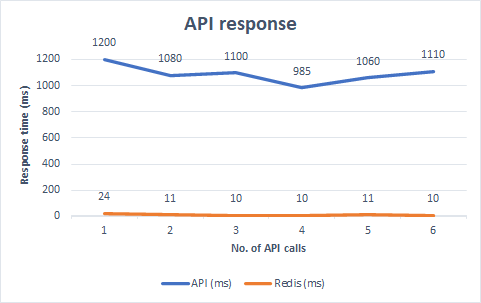
\includegraphics{images/Grafico.png}
    \caption{Comparação dos tempos de resposta da API com e sem Redis Cache}
    \label{fig:my_label}
\end{figure}

\section{Conclusão}

Através da realização deste trabalho de análise, consistindo na idealização, desenvolvimento e avaliação de um modelo de aplicação, foi possível obter valiosas informações a respeito do funcionamento e comportamento do Redis como um Sistema de Cache em um sistema real. Partindo de uma ideia simples, que é o consumo de uma API externa atuando como uma espécie de proxy, permitindo a interceptação e armazenamento dos dados trafegados foi extremamente importante, garantindo assim o êxito nos testes e a compreensão total do real impacto deste middleware.

Com base nos números obtidos, ficam claros os benefícios da utilização não apenas do Redis, mas de qualquer middleware de cache em cenários de Sistemas Distribuídos, embora o Redis possua notoriedade e demonstre-se expressivamente mais ágil e performático, quase que absolutamente.

No caso de exemplo elaborado e descrito neste artigo, a difícil mutabilidade nos dados retornados trazia consigo características clássicas de aptidão para uso de armazenamento cache, o que ficou explícito nos resultados apresentados, diminuindo em cem vezes o tempo entre o recebimento de uma demanda e o retorno das informações desejadas a um cliente.

Por fim,é importante reconhecer que nenhuma tecnologia é uma "bala de prata", e que o sucesso de seu emprego em projetos reais depende de inúmeros fatores, que tornam ou não uma ferramenta adequada para um sistema. 

\end{document}
